\begin{figure}[h]
	\centering
    \begin{tikzpicture}
    \node[inner sep=0pt] (pic) at (0,0)
    {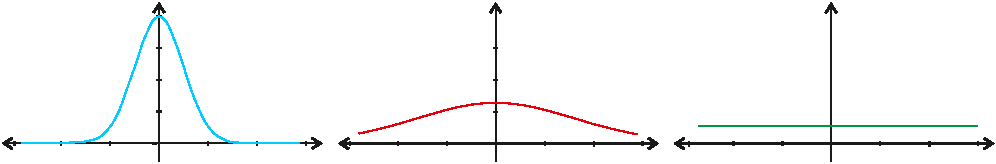
\includegraphics[width=15.5cm]{pictures/picture_2_4.pdf}};
    \draw [color=black](4.6,-0.2) node[anchor=north west] {$ c $};
    \draw [color=black](0,-1) node[anchor=north west] {$ \mu_{0} $};
    \draw [color=black](-5.2,-1) node[anchor=north west] {$ \mu_{0} $};
    \draw [color=black](-4.5,0.5) node[anchor=north west] {$ \sigma^{2} = 1 $};
    \draw [color=black](1,0.5) node[anchor=north west] {$ \sigma^{2} = 10 $};
    \draw [color=black](6,0.5) node[anchor=north west] {$ \sigma^{2} \rightarrow \infty $};
    \end{tikzpicture}
    \caption{Vykreslení změny normálního rozdělení při rostoucím rozptylu.}
\end{figure}